\documentclass[conference]{IEEEtran}
\usepackage{cite}
\usepackage{amsmath,amssymb}
\usepackage{booktabs}
\usepackage{graphicx}
\usepackage{url}
\title{Decision-Threshold Selection and Zero-Noise Extrapolation in Variational Quantum Classifiers under Simulated Noise}
\author{\IEEEauthorblockN{Author 1, Author 2, Author 3}\IEEEauthorblockA{Affiliations: \\ Corresponding author email: }}
\begin{document}
\maketitle
\begin{abstract}
We compare held-out threshold selection with probability-scaled zero-noise extrapolation (ZNE) for noiselessly trained variational quantum classifiers under matched simulated measurement budgets including calibration. On standardized-PCA WDBC at $\gamma=0.30$, exact calibrated balanced accuracy is 0.878; with 1,000 measurements it is 0.778, versus 0.716 for linear ZNE and 0.582 for quadratic ZNE. In a post-hoc sweep, 10 labeled calibration examples recover most of the gain (0.760 balanced accuracy versus 0.783 with all 114). Gate-folded ZNE at scales 1, 3, and 5 reaches 0.682 under the same budget, below noisy-threshold calibration. In a local IBM FakeManilaV2 snapshot simulation, fixed-threshold classification remains near clean performance, while readout correction and gate-folded ZNE produce changes within checkpoint variability; this is not a hardware run. Standardized transfer runs on the same saved splits show a similar tested-pipeline ordering on Wine and balanced synthetic data; matched clean logistic regression exceeds the quantum model on these tasks. A post-hoc depth sweep and score-spread diagnostic is consistent with 1-layer circuits retaining a wider class-score gap (0.210 vs 0.079 vs 0.008), which prevents measurement shot noise from swamping the class boundary. Results establish neither hardware advantage nor clinical validity.\end{abstract}
\begin{IEEEkeywords}
quantum machine learning, variational quantum classifier, zero-noise extrapolation, decision threshold, finite-shot measurement, error mitigation
\end{IEEEkeywords}

\section{Introduction and related work}
Noise robustness in quantum classification has been studied through robust data encodings and channel-dependent decision boundaries~\cite{larose2020}. QuantumNAT analyzes noise-induced score scaling and shifts, normalization, and noise-aware training~\cite{wang2022}. Decision-threshold selection and probability calibration are distinct established operations~\cite{hernandez2012,niculescu2005}: here ``calibration'' means selecting a decision threshold for balanced accuracy on held-out labels, not fitting calibrated posterior probabilities. Richardson zero-noise extrapolation was introduced for short-depth circuits and later developed for variational and digital circuits~\cite{temme2017,libenjamin2017,giurgica2020}; broader mitigation methods and limitations are reviewed by Cai et al.~\cite{cai2023}. ZNE implementation has known subtleties~\cite{majumdar2023}, including finite-shot help--harm effects~\cite{koester2026,scavino2026}. Our question is operational: for a fixed total measurement budget including labeled calibration measurements, how do label-dependent threshold selection and label-free probability-scaled ZNE compare in thresholded classifier performance? The contributions are: (1) a matched-budget comparison that counts calibration measurements; (2) a calibration-size sensitivity analysis and a depth diagnostic linking score separation to shot uncertainty; and (3) an analysis separating exact observable bias, finite-shot sampling error, decision-rule fitting variability, and classification performance, with paired comparisons across held-out folds. We do not propose a new mitigation estimator or claim a universal ranking, hardware validation, or quantum advantage.

\section{Question and model}
We ask: when a noisy classifier predicts one class, how much can held-out threshold or affine calibration recover, and how does finite measurement precision affect recovery relative to linear and quadratic ZNE? The classifier encodes $d=n$ PCA features by $R_X(x_j)$ rotations, applies trainable $R_Y$ and $R_Z$ rotations with a CNOT-chain, CZ-ring, or readout-centered CNOT-star entangler, and measures $z=\langle Z_0\rangle\in[-1,1]$. The training objective uses $\sigma(z)$ with binary cross-entropy; this sigmoid is a training parameterization and is not interpreted as a calibrated patient probability. Classification at the fixed boundary uses $z\geq0$.

For a final amplitude-damping channel immediately before measurement, the standard Bloch-coordinate relation is $z_{\rm out}=(1-\gamma)z_{\rm in}+\gamma$; it illustrates how a positive offset can move scores across a fixed threshold while preserving their ranking for $\gamma<1$. The relation is not assumed for the interleaved circuit studied here. Depolarizing noise and phase damping are modeled as distinct channels. All $\gamma$ values in our simulator denote probabilities at declared channel locations, not an overall circuit error rate or device $T_1/T_2$ times.

\section{Experimental design}
For WDBC the target labels are malignant (0) and benign (1). Tasks are the UCI Wisconsin Diagnostic Breast Cancer dataset (WDBC)~\cite{wdbc}, the UCI Wine dataset reduced to class 0 versus classes 1/2~\cite{wine}, and two scikit-learn synthetic tasks generated with fixed seeds (600 samples, 12 features, 6 informative, 2 redundant, 2 clusters per class, class separation 1.0; seeds 1729/1730 and class weights 0.5/0.5 or 0.8/0.2)~\cite{sklearn}. Table~\ref{tab:datasets} reports dataset sizes, counts, partition sizes, and PCA variance for the secondary unstandardized pipeline; the standardized primary variances are also listed. Each task uses 5 stratified folds with disjoint test sets; the initial 60/20/20 model-training-pool/calibration/test split is further divided 85/15 into weight-fit and development data. All preprocessing is fit on the outer training pool before its 85/15 weight-fit/development split; calibration and test data are held out from preprocessing. The primary pipeline standardizes features before two-component PCA. 2 training initializations are used per fold. The four-qubit CNOT-star used for broader comparisons passed a random-weight feature-dependence probe. The primary two-qubit CNOT and CZ circuits also passed post-hoc probes confirming both encoded inputs can affect their readouts. Channel controls use differing noise locations and are descriptive, not causal.

Models are trained without noise on PennyLane's \texttt{default.qubit} simulator using Adam (learning rate 0.1), binary cross-entropy on $\sigma(\langle Z_0\rangle)$, uniform $[-\pi,\pi]$ initialization, batch size 32, and 30 epochs. The two-qubit model has eight trainable angles. Development examples are monitored but do not select checkpoints; the last epoch is evaluated. This is a noise-unaware training study, with noisy evaluation on PennyLane \texttt{default.mixed}. The recorded environment is Python 3.12.14, PennyLane 0.43.3, NumPy 2.2.6, pandas 2.3.3, and scikit-learn 1.7.2 on Windows 11. Training histories are reported; they are not evidence of convergence.

At each composite-noise test setting, we evaluate exact expectations and finite shots. In the primary analysis, ZNE scale factors multiply the declared channel probabilities in the simulator; this is probability-scaled Richardson extrapolation, not gate folding or hardware noise scaling. A separate gate-folding simulator sensitivity is reported below; neither analysis is a hardware result. The fixed threshold and uncalibrated ZNE use the full nominal per-case budget for inference. Clean-frozen calibration, noisy threshold calibration, affine readout, and calibrated ZNE divide the nominal budget between independent calibration and test examples; because counts are integer and fold sizes may differ, realized totals vary by at most 0.443\% from the fixed-threshold total. Actual shot costs are saved. Clean-frozen thresholds are estimated from clean finite-shot calibration scores and held fixed across noise settings. Noisy thresholds and ZNE thresholds are fit on their respective calibration scores only. Linear ZNE uses scales $\{1,2\}$ and coefficients $(2,-1)$; quadratic ZNE uses scales $\{1,1.5,2\}$ and coefficients $(6,-8,3)$. ZNE shots are allocated in proportion to absolute coefficients. We distinguish observable error relative to the clean expectation from classification recovery under a changed decision rule. Following standard finite-shot ZNE analyses~\cite{scavino2026,mohammadipourli2025}, for independent Pauli-$Z$ sample means at scales $s_i$, the Richardson estimate is $\hat z=\sum_i c_i\hat\mu_i$, with $\mathrm{Var}(\hat z)=\sum_i c_i^2(1-\mu_i^2)/n_i$. Under a total of $N=\sum_i n_i$ shots, the variance-minimizing allocation is $n_i\propto |c_i|\sqrt{1-\mu_i^2}$; when per-shot variances are treated as equal, this reduces to allocation proportional to $|c_i|$, as used here. The resulting worst-case variance bound is $(\sum_i|c_i|)^2/N$. We recall this standard estimator-level bound rather than claim it as a new result. The linear $(2,-1)$ rule has bound $9/N$, the quadratic $(6,-8,3)$ rule has $289/N$, and the exploratory $(15,-24,10)$ rule has $2401/N$. This estimator-level variance result does not determine classification accuracy or a universal crossover against calibration: that also depends on score distributions, calibration labels, and threshold-fit uncertainty. We do not claim such a crossover theorem.

We report accuracy, balanced accuracy, per-class recall, ROC-AUC, confusion counts, predicted class fraction, observable error, shot cost, and single-class prediction frequency. Paired contrasts are calculated on matched model/test splits. Fold-level summaries are descriptive under the repeated-split protocol; test sets overlap and are not independent populations.

The separate gate-folding sensitivity implements each primitive gate using an alternating odd-fold sequence $U$, $U^{-1}$, $U$, and so on, with 1, 3, or 5 physical occurrences, and applies the same declared composite channel after each physical gate occurrence. Richardson coefficients are $(15/8,-5/4,3/8)$; with a 1,000-measurement per-case budget, 500 measurements are allocated to calibration and 500 to inference, divided across scales in proportion to the absolute coefficients. The experiment reuses the 10 standardized WDBC checkpoints and five saved folds and averages 20 finite-shot draws. The scale-one circuit reproduces the original exact composite-channel scores to numerical precision. This is a simulator gate-folding study under an assumed gate-local channel, not a hardware execution.

\section{Results}
\subsection{Primary WDBC matched-budget comparison with standardized PCA}
The primary WDBC matched-budget comparison standardizes each feature on the outer training pool, then fits two-component PCA, and uses the same five outer folds and two initialization seeds. The components retain 0.634 of variance. At zero noise, quantum fixed-threshold balanced accuracy is 0.887; logistic regression on the same standardized two components reaches 0.928, so the classical matched-input model is stronger. At $\gamma=0.30$, exact threshold fitting gives 0.878; exact calibrated linear and quadratic ZNE give 0.883 and 0.884. Under the matched 1,000-shot budget, noisy threshold calibration gives 0.778, compared with linear ZNE plus calibration at 0.716 and quadratic ZNE plus calibration at 0.582; calibrated methods divide the nominal budget between calibration and test inference. The five fold-level threshold-minus-ZNE differences are +0.071, +0.071, +0.052, +0.052, +0.065 for linear and +0.210, +0.199, +0.200, +0.191, +0.179 for quadratic ZNE. All five folds have the same sign, but folds overlap and this is descriptive variability, not independent-population evidence.
Table~\ref{tab:primary-gatefold} reports the separate gate-folded simulator comparison: scales 1, 3, and 5 give balanced accuracy 0.682 under the same nominal budget. Its scale-one circuit matches the original composite-channel expectation within $2.3\times10^{-16}$. It uses the saved checkpoints and folds and is not hardware validation.
\begin{table*}[t]\centering\scriptsize
\caption{Standardized-PCA WDBC results at $\gamma=0.30$. Thresholds use calibration labels only. The nominal finite-shot budget is 1,000 measurements per test case, split between calibration and test inference. Finite-shot means average 20 draws per checkpoint; reported SD is across the 10 checkpoint means, which are nested in five overlapping folds.}
\label{tab:standardized}
\begin{tabular}{@{}l r r r@{}}\toprule
Pipeline & Balanced accuracy & ROC-AUC & $n$ \\
\midrule
Quantum, clean fixed threshold & 0.887 $\pm$ 0.035 & 0.958 & 10 \\
Quantum, clean threshold fit & 0.882 $\pm$ 0.027 & 0.958 & 10 \\
Quantum, exact noisy fixed ($\gamma=0.30$) & 0.500 $\pm$ 0.000 & 0.958 & 10 \\
Quantum, exact noisy threshold fit & 0.878 $\pm$ 0.027 & 0.958 & 10 \\
Logistic regression, same standardized 2D inputs & 0.928 $\pm$ 0.026 & 0.989 & 10 \\
Linear ZNE, exact, threshold fit & 0.883 $\pm$ 0.028 & 0.958 & 10 \\
Quadratic ZNE, exact, threshold fit & 0.884 $\pm$ 0.028 & 0.958 & 10 \\
Noisy score, 1,000 shots, fixed threshold & 0.503 $\pm$ 0.003 & 0.868 & 10 \\
Noisy threshold fit, 1,000 shots & 0.778 $\pm$ 0.014 & 0.868 & 10 \\
Linear ZNE, 1,000 shots, fixed threshold & 0.583 $\pm$ 0.012 & 0.799 & 10 \\
Linear ZNE, 1,000 shots, threshold fit & 0.716 $\pm$ 0.012 & 0.799 & 10 \\
Quadratic ZNE, 1,000 shots, fixed threshold & 0.587 $\pm$ 0.006 & 0.633 & 10 \\
Quadratic ZNE, 1,000 shots, threshold fit & 0.582 $\pm$ 0.008 & 0.633 & 10 \\
\bottomrule\end{tabular}\end{table*}
Figure~\ref{fig:headline} summarizes the primary matched-budget comparison. Error bars are descriptive SD across 10 checkpoint means nested in five overlapping folds.
\begin{figure*}[t]\centering
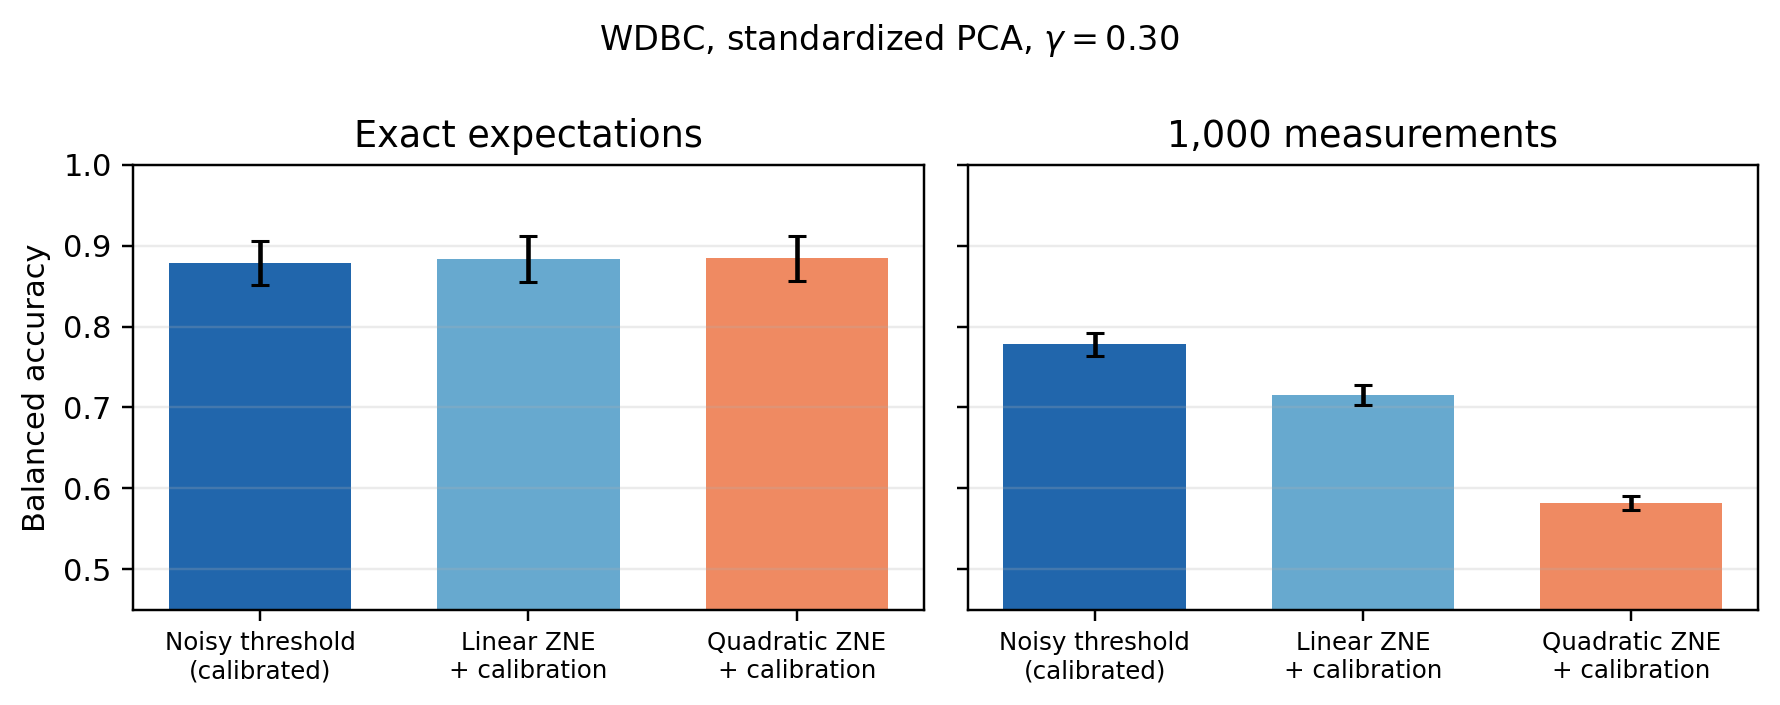
\includegraphics[width=0.78\textwidth]{headline_primary_wdbc.png}
\caption{Primary standardized-PCA WDBC comparison at $\gamma=0.30$. Bars show balanced accuracy for noisy-threshold calibration and calibrated linear/quadratic ZNE under exact expectations and a 1,000-measurement budget. Error bars show descriptive SD across 10 checkpoint means; checkpoints are nested in five overlapping folds.}
\label{fig:headline}\end{figure*}
\begin{figure}[t]\centering
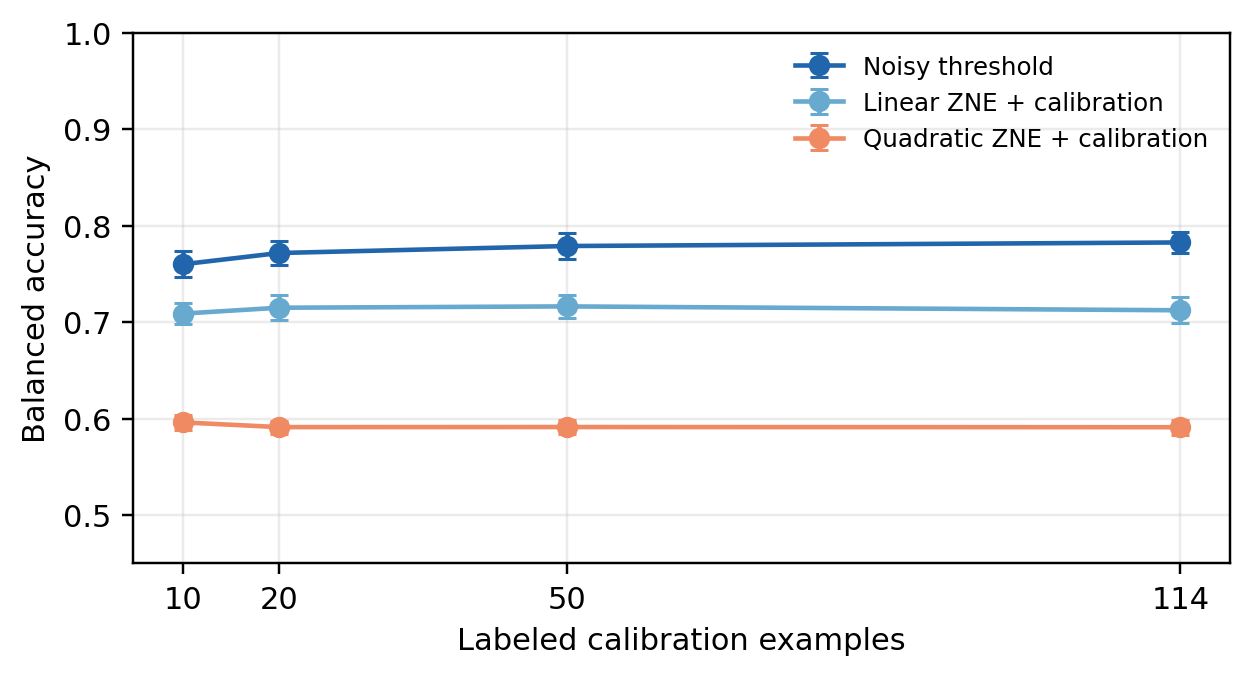
\includegraphics[width=0.98\columnwidth]{calibration_efficiency_wdbc.png}
\caption{Post-hoc calibration-size sensitivity for standardized-PCA WDBC at $\gamma=0.30$. Points average 20 shot draws within each of 10 checkpoints; error bars are SD across checkpoint means nested in five overlapping folds.}
\label{fig:calsize}\end{figure}

A post-hoc calibration-size sensitivity (Fig.~\ref{fig:calsize}) gives noisy-threshold balanced accuracy 0.760 with 10 labels and 0.783 with 114 under a nominal 1,000-measurement budget. The 114-label mean differs slightly from the main table (0.778) because this sweep uses an independent calibration-shot RNG stream; the folds, checkpoints, 114 labels, test draws, and threshold rule are held fixed. This is a reused-checkpoint sensitivity analysis, not independent validation.
At $\gamma=0.30$, finite-shot calibrated balanced accuracy is 0.854 at one layer, 0.778 at the two-layer primary depth, and 0.525 at four layers (Table~\ref{tab:primary-depth}). A post-hoc calibration-score diagnostic finds class-mean gaps of 0.210, 0.079, and 0.008 at depths 1, 2, and 4; the class gap contracts roughly $\times 0.38$ from layer 1 to 2 and $\times 0.11$ from layer 2 to 4 (about $\times 0.32$ per layer). Because Pauli-$Z$ measurement standard error scales as $\sigma/\sqrt{N}$ (about 0.043 at 500 shots for all depths), matching the depth-1 signal-to-noise ratio (SE/gap $= 0.328$) at depth 4 would require $N \propto 1/\text{gap}^2$, or $(0.210 / 0.0083)^2 \approx 640\times$ more shots (over 320,000 measurements). At 500 shots, the sampling SE (0.043) is more than five times larger than the depth-4 class gap (0.008), completely swamping the decision boundary in finite-shot noise. This quantitative signal-to-noise scaling explains the depth collapse without invoking a universal depth law; two layers were fixed as primary before this sweep.
An exact-expectation sweep on the same standardized-PCA checkpoints covers $\gamma=0.0$--$0.4$; at $\gamma=0.30$, the fixed threshold gives 0.500 balanced accuracy and held-out threshold selection gives 0.878. Supplementary Table~S15 reports the complete grid, including calibrated ZNE. This reuses the primary folds and checkpoints.
Table~\ref{tab:primary-transfer} reports standardized-PCA runs on the same saved splits and initialization seeds for WDBC, Wine, and balanced synthetic data. Each row averages 20 finite-shot draws per checkpoint at $\gamma=0.30$ and a nominal 1,000-measurement budget; repeated draws and overlapping folds are descriptive, not independent task replications. Clean matched-input logistic regression reaches 0.928 on WDBC, 0.950 on Wine, and 0.747 on balanced synthetic data; it exceeds clean quantum performance on all three.
Table~\ref{tab:fake-backend} reports a local simulation using the saved IBM FakeManilaV2 Falcon r5.11 backend snapshot (Qiskit 2.5.2, Aer 0.17.2, optimization level 0, physical qubits [0, 1]); the saved snapshot is not current calibration data and no QPU was executed. Under a matched 1,000-measurement budget (500 calibration, 500 test), the raw fixed threshold reaches balanced accuracy 0.886, matching the clean model (0.887). Held-out calibration yields 0.873, readout mitigation yields 0.885 (fixed) and 0.878 (calibrated), and gate-folded ZNE yields 0.877 (fixed) and 0.885 (calibrated). All evaluated methods sit within 0.013 of one another, well within checkpoint standard deviations (0.025--0.038). Readout-mitigated and raw ROC-AUC are both 0.958 to the reported precision. Balanced-accuracy differences are small relative to checkpoint variability, so this experiment does not show a consistent incremental classification benefit from readout correction. In this snapshot setting, no boundary collapse appears. The post-hoc noise-multiplier sweep (Fig.~\ref{fig:regime-map}) is an exploratory stress test: threshold calibration remains comparatively stable while gate-folded ZNE degrades at the highest tested multiplier. Neither result establishes a general ranking.

\subsection{Secondary unstandardized-PCA analyses}
The earlier unstandardized-PCA noise grids, channel controls, and cross-task comparisons are retained as secondary analyses in the supplementary material. They are not used to estimate the primary standardized-PCA result.

\subsection{Clean performance and classical controls}
Table~\ref{tab:datasets} reports the task definitions and partition sizes. Table~\ref{tab:classical} compares the quantum model with classical controls using the same two PCA inputs and with full-feature controls. It reports both an outer-training-pool logistic model and a logistic model fit on the exact weight-fit examples used by each quantum initialization. All classical decisions use the default 0.5 threshold. The matched-fit comparison isolates input representation and fits on the same example count; the larger-pool baseline reflects the full outer training data available before calibration.
\begin{table*}[t]\centering\scriptsize
\caption{Task definitions and partition sizes. PCA variance columns distinguish the secondary unstandardized pipeline from standardized-before-PCA controls; the imbalanced task has no standardized transfer run.}
\label{tab:datasets}
\begin{tabular}{@{}l r r l l r r@{}}\toprule
Task & $n$ & Features & Class counts & Fit/dev/cal/test ranges & Raw PCA var. & Std. PCA var. \\
\midrule
WDBC & 569 & 30 & 212/357 & 289--290/52/114/113--114 & 0.998 & 0.634 \\
Wine 0 vs rest & 178 & 13 & 59/119 & 90/16--17/36/35--36 & 1.000 & 0.549 \\
Synthetic balanced & 600 & 12 & 300/300 & 306/54/120/120 & 0.573 & 0.360 \\
Synthetic imbalanced & 600 & 12 & 478/122 & 306/54/120/120 & 0.681 & -- \\
\bottomrule\end{tabular}\end{table*}
\begin{table*}[t]\centering\scriptsize
\caption{Clean balanced accuracy: quantum model and classical controls across standardized and raw PCA pipelines. Standardized 2D inputs are directly comparable (Quantum 0.887 vs Logistic 0.928 on WDBC; 0.858 vs 0.950 on Wine; 0.689 vs 0.747 on balanced synthetic). Secondary unstandardized 2D and full-feature classical baselines are reported for comparison. All classical decisions use a fixed 0.5 threshold.}
\label{tab:classical}
\begin{tabular}{@{}l r r r r r r r r@{}}\toprule
Task & Quantum 2D (std.) & Quantum 2D (raw) & Logistic 2D (std.) & Logistic 2D (raw) & Logistic 2D matched fit $n$ & Logistic full & RBF SVM full & Random forest full \\
\midrule
WDBC & 0.887 & 0.812 & 0.928 & 0.904 & 0.902 & 0.966 & 0.966 & 0.948 \\
Wine 0 vs rest & 0.858 & 0.850 & 0.950 & 0.907 & 0.909 & 0.992 & 0.992 & 0.979 \\
Synthetic balanced & 0.689 & 0.697 & 0.747 & 0.782 & 0.782 & 0.837 & 0.848 & 0.853 \\
Synthetic imbalanced & -- & 0.526 & -- & 0.502 & 0.502 & 0.686 & 0.731 & 0.635 \\
\bottomrule\end{tabular}\end{table*}
Table~\ref{tab:classicalpaired} reports paired quantum-minus-logistic differences for the exact fit-size-matched rows. Its intervals are descriptive bootstraps over five fold means, not population-level confidence intervals.
\begin{table}[t]\centering\small
\caption{Paired clean balanced-accuracy contrasts: quantum 2D model minus fit-size-matched 2D logistic regression.}
\label{tab:classicalpaired}
\begin{tabular}{@{}l r l r@{}}\toprule
Task & Difference & Descriptive 95\% interval & Folds \\
\midrule
Synthetic balanced & -0.085 & [-0.127, -0.048] & 5 \\
Synthetic imbalanced & +0.024 & [-0.034, +0.078] & 5 \\
WDBC & -0.089 & [-0.118, -0.064] & 5 \\
Wine 0 vs rest & -0.060 & [-0.136, +0.003] & 5 \\
\bottomrule\end{tabular}\end{table}
Across saved model runs, clean-expectation two-qubit balanced accuracy / ROC-AUC were: WDBC: 0.812 balanced accuracy / 0.959 ROC-AUC; Wine class 0 vs rest: 0.850 balanced accuracy / 0.930 ROC-AUC; balanced synthetic: 0.697 balanced accuracy / 0.766 ROC-AUC; imbalanced synthetic: 0.526 balanced accuracy / 0.462 ROC-AUC. The imbalanced synthetic task remains a negative result: its quantum AUC is near chance (0.462) and its clean balanced accuracy is weak (0.526), while full-feature classical baselines achieved logistic\_regression\_full 0.686 balanced accuracy; random\_forest\_full 0.635 balanced accuracy; rbf\_svm\_full 0.731 balanced accuracy. Per-epoch training and development curves are saved; the per-task median optimizer updates were Synthetic balanced 300; Synthetic imbalanced 300; WDBC 300; Wine 0 vs rest 90 over 30 epochs at batch size 32. We retain the weak task as a failed diagnostic, not evidence that mitigation preserves a functioning classifier. WDBC and Wine classical baselines also exceed the two-qubit model in this pilot, so no comparative predictive advantage is claimed.


Figure~\ref{fig:training} shows the training and development histories. WDBC and Wine losses decline and then change less across later epochs; the balanced synthetic task improves modestly, while imbalanced synthetic development performance remains near chance. We use the fixed 30-epoch protocol and do not treat these curves as proof of convergence.
\begin{figure*}[t]
\centering
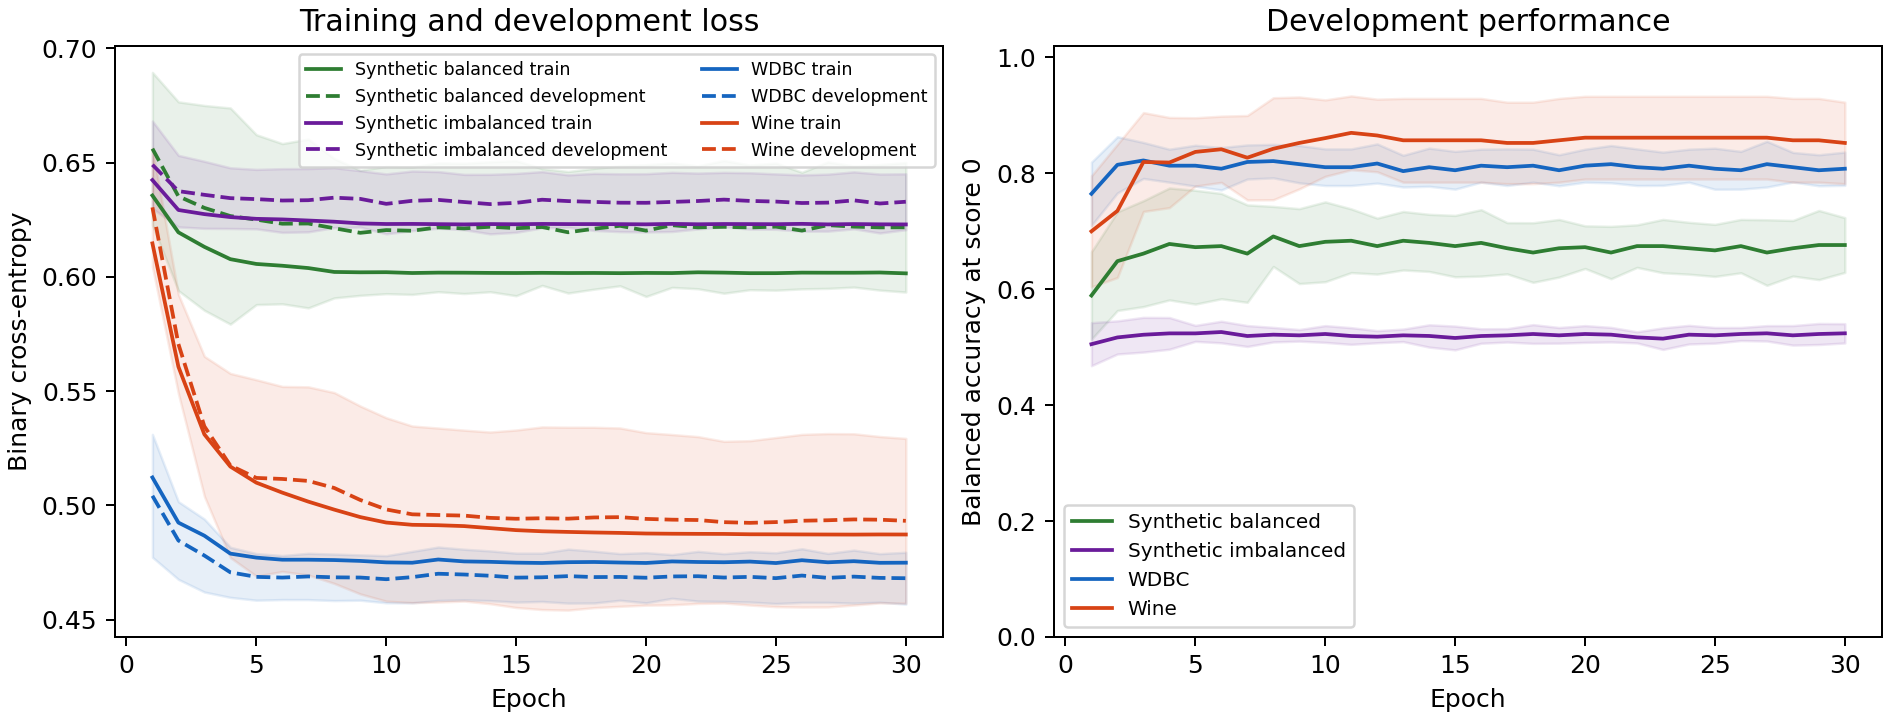
\includegraphics[width=0.82\textwidth]{training_convergence.png}
\caption{Training and development binary cross-entropy and development balanced accuracy at the fixed threshold, averaged over 5 folds for the core two-qubit CNOT-chain models. Shading shows fold-level standard deviation after averaging initializations within each fold.}
\label{fig:training}
\end{figure*}

\subsection{Paired comparisons in the primary pipeline}
Table~\ref{tab:primary-paired} reports the fold-level difference in balanced accuracy for the standardized WDBC pipeline at $\gamma=0.30$ and 1,000 measurements (ZNE minus noisy-threshold calibration). Each value is computed after averaging the matched shot draws within the corresponding fold and initialization. Fold test sets overlap, so these five values describe protocol variability rather than independent replicates. Across 10 checkpoint means (nested within five overlapping folds), exploratory one-sided Wilcoxon signed-rank diagnostics are linear: nominal one-sided exact $p=0.0010$ and quadratic: nominal one-sided exact $p=0.0010$; the nominal values are not treated as independent-population inference.
\begin{table*}[t]\centering\small
\caption{Primary standardized-PCA WDBC fold-level paired contrasts, $\gamma=0.30$, nominal budget 1,000. Entries are ZNE minus noisy-threshold calibrated balanced accuracy; negative values favor threshold calibration.}
\label{tab:primary-paired}
\begin{tabular}{@{}l r r r r r r@{}}\toprule
Method & Fold 1 & Fold 2 & Fold 3 & Fold 4 & Fold 5 & Mean \\
\midrule
Linear ZNE & -0.071 & -0.071 & -0.052 & -0.052 & -0.065 & -0.062 \\
Quadratic ZNE & -0.210 & -0.199 & -0.200 & -0.191 & -0.179 & -0.196 \\
\bottomrule\end{tabular}\end{table*}
\subsection{Supplementary paired and sensitivity analyses}
Full paired contrasts for the legacy unstandardized pipeline, calibration-allocation variants, and ZNE scale schedules are provided in the supplementary tables. These post-hoc analyses reuse the recorded folds.

\subsection{Score and budget diagnostics}
Secondary unstandardized-PCA noise-grid, finite-budget, and architecture diagnostics appear in Supplementary Figures~S1--S3 and Tables~S1--S17. The primary two-qubit CNOT-chain and CZ-ring circuits, and the four-qubit CNOT-star, passed a finite random-weight feature-to-readout probe for every encoded input. This probe establishes only sensitivity under tested perturbations, not useful learning or scaling. The single four- and six-qubit CNOT-chain controls had weak or absent feature dependence and remain architecture diagnostics; there is no four-qubit CZ-ring model in this study.




\subsection{Scope of the secondary synthetic diagnostic}
The separate weak-signal synthetic task-family diagnostic is retained in the supplementary archive as a negative result; its near-chance baseline is not used as confirmation of the main finding.

\begin{table*}[t]\centering\scriptsize
\caption{Post-hoc standardized-PCA WDBC depth and score-separation diagnostic at $\gamma=0.30$. Clean and exact-noisy metrics are checkpoint means. Finite-shot balanced accuracy averages 20 draws per checkpoint; its SD is across checkpoint means. Score spread, clean-shot gap, and one-score sampling SE are computed on calibration observations; folds overlap.}
\label{tab:primary-depth}
\begin{tabular}{@{}r r r r r r r r r@{}}\toprule
Layers & Clean BA & Exact noisy BA & Finite BA $\pm$ SD & Finite AUC & Score SD & Class gap & SE at 500 & SE/gap \\ \midrule
1 & 0.873 & 0.849 & 0.854 $\pm$ 0.031 & 0.929 & 0.132 & 0.210 & 0.043 & 0.206 \\
2 & 0.887 & 0.878 & 0.778 $\pm$ 0.014 & 0.868 & 0.047 & 0.079 & 0.044 & 0.558 \\
4 & 0.885 & 0.873 & 0.525 $\pm$ 0.007 & 0.549 & 0.005 & 0.008 & 0.043 & 5.136 \\
\bottomrule\end{tabular}\end{table*}

\begin{table*}[t]\centering\small
\caption{Standardized-PCA finite-shot transfer comparison on the same saved splits and initialization seeds, $\gamma=0.30$, nominal budget 1,000. Threshold calibration includes its measurement cost. Values average 20 draws per checkpoint; no error bars are shown because the rows are descriptive and nested within five overlapping folds.}
\label{tab:primary-transfer}
\begin{tabular}{@{}l r r r r@{}}\toprule
Task & Fixed threshold & Noisy threshold + calibration & Linear ZNE + calibration & Quadratic ZNE + calibration \\ \midrule
WDBC (standardized PCA) & 0.503 & 0.778 & 0.716 & 0.582 \\
Wine, class 0 vs rest & 0.500 & 0.701 & 0.650 & 0.557 \\
Synthetic, balanced & 0.500 & 0.612 & 0.584 & 0.534 \\
\bottomrule\end{tabular}\end{table*}

\begin{table*}[t]\centering\small
\caption{Matched-budget standardized-PCA WDBC finite-shot comparison at $\gamma=0.30$. Each calibrated pipeline uses 500 measurements per calibration example and 500 per test case in total, with scale shots allocated proportionally to absolute Richardson coefficients. Means are over 20 draws per saved checkpoint; SD is across 10 checkpoint means nested in five overlapping folds. Its calibrated baseline (0.776 $\pm$ 0.020) uses independent shot seeds from the main table (0.778 $\pm$ 0.022).}
\label{tab:primary-gatefold}
\begin{tabular}{@{}l r r r@{}}\toprule
Pipeline & Balanced accuracy $\pm$ checkpoint SD & ROC-AUC & Checkpoints \\ \midrule
Noisy threshold + calibration & 0.776 $\pm$ 0.020 & 0.863 & 10 \\
Gate-folded ZNE + calibration & 0.682 $\pm$ 0.016 & 0.757 & 10 \\
Probability-scaled linear ZNE + calibration & 0.716 $\pm$ 0.012 & 0.799 & 10 \\
Probability-scaled quadratic ZNE + calibration & 0.582 $\pm$ 0.008 & 0.633 & 10 \\
\bottomrule\end{tabular}\end{table*}

\begin{table*}[t]\centering\small
\caption{IBM FakeManilaV2 device-model evaluation on standardized WDBC at nominal budget 1,000 (500 calibration, 500 test). Single-qubit readout error mitigation uses calibration matrix inversion on qubit 0. Gate-folded ZNE uses scales 1, 3, 5 with Richardson coefficients $(15/8, -5/4, 3/8)$ transpiled with non-canceling unitary folding. SDs are across 10 checkpoint means nested in five overlapping folds.}
\label{tab:fake-backend}
\begin{tabular}{@{}l r r r@{}}\toprule
Method & Balanced accuracy $\pm$ checkpoint SD & ROC-AUC & Checkpoints \\ \midrule
Raw device noise, fixed threshold & 0.886 $\pm$ 0.038 & 0.958 & 10 \\
Raw device noise, calibrated & 0.873 $\pm$ 0.027 & 0.958 & 10 \\
Readout mitigation, fixed & 0.885 $\pm$ 0.038 & 0.958 & 10 \\
Readout mitigation, calibrated & 0.878 $\pm$ 0.031 & 0.958 & 10 \\
Gate-folded ZNE, fixed & 0.877 $\pm$ 0.033 & 0.952 & 10 \\
Gate-folded ZNE, calibrated & 0.885 $\pm$ 0.025 & 0.952 & 10 \\
Readout mitigation + gate-folded ZNE, cal. & 0.885 $\pm$ 0.025 & 0.952 & 10 \\
\bottomrule\end{tabular}\end{table*}

\section{Discussion and limitations}
The study's conclusions are limited to its simulator settings and saved folds:
\begin{itemize}
\item The main matched-budget comparison is standardized-PCA WDBC, with standardized-PCA transfer runs on the same saved splits and initialization seeds for Wine and balanced synthetic data; legacy broad noise-grid controls use unstandardized PCA and are secondary.
\item The five outer folds overlap, and both transfer tasks reuse those split and initialization seeds; these results do not provide broad population-level validation.
\item Threshold fitting uses held-out labels and consumes measurements, so performance may depend on calibration-set size and shot allocation.
\item Classical logistic regression on the same standardized inputs reaches 0.928 clean balanced accuracy, above the quantum model's 0.887; no predictive advantage is shown.
\item Training is noiseless and fixed at 30 epochs. The primary ZNE comparison scales simulated channel probabilities; a separate matched-budget gate-folded simulator sensitivity is reported. The device-model evaluation uses a single fake-backend snapshot; no real-hardware run was performed.
\end{itemize}
The results do not establish clinical performance, quantum advantage, or a general ranking of mitigation methods.

Same-environment retraining without checkpoint reuse reproduced all 56 model configurations bitwise and matched 37216 exact/finite-shot metrics (maximum difference 0.0e+00) plus 5040 training-curve values; this verifies deterministic rerun reproducibility on the recorded environment, not external validation.

The implementation saves split indices, frozen weights, preprocessing objects, per-example observations, package versions, and configuration hashes. Code, figures, and saved result artifacts are included in the accompanying project archive. The device-model evaluation uses a single fake-backend snapshot; no real-hardware or probabilistic-error-cancellation run was performed.

\section{Conclusion}
In this simulator study, held-out threshold selection improves classification over the fixed boundary in the standardized WDBC setting, but finite-shot recovery is incomplete and the tested ZNE result depends on schedule and budget. Ten calibration labels reach balanced accuracy 0.760 in the post-hoc sensitivity analysis, compared with 0.783 using all 114 labels. Performance also declines across the tested depth sweep, alongside a sharp reduction in noisy class-score separation. Transfer runs on the same saved Wine and balanced-synthetic splits show the same tested-pipeline ordering, while clean matched logistic baselines remain stronger on WDBC and Wine. These bounded observations motivate device-aware and readout-mitigation comparisons; they do not establish general superiority or quantum advantage.

\begin{thebibliography}{99}
\bibitem{hernandez2012} J. Hern\'andez-Orallo, P. Flach, and C. Ferri, ``A unified view of performance metrics: Translating threshold choice into expected classification loss,'' \emph{Journal of Machine Learning Research}, vol. 13, pp. 2813--2869, 2012.
\bibitem{niculescu2005} A. Niculescu-Mizil and R. Caruana, ``Predicting good probabilities with supervised learning,'' in \emph{Proc. 22nd International Conference on Machine Learning}, pp. 625--632, 2005, doi: 10.1145/1102351.1102430.
\bibitem{temme2017} K. Temme, S. Bravyi, and J. M. Gambetta, ``Error mitigation for short-depth quantum circuits,'' \emph{Physical Review Letters}, vol. 119, 180509, 2017.
\bibitem{libenjamin2017} Y. Li and S. C. Benjamin, ``Efficient variational quantum simulator incorporating active error minimization,'' \emph{Physical Review X}, vol. 7, 021050, 2017.
\bibitem{cai2023} Z. Cai et al., ``Quantum error mitigation,'' \emph{Reviews of Modern Physics}, vol. 95, 045005, 2023.
\bibitem{wdbc} W. H. Wolberg, W. N. Street, and O. L. Mangasarian, ``Breast Cancer Wisconsin (Diagnostic),'' UCI Machine Learning Repository, DOI: 10.24432/C5DW2B.
\bibitem{wine} S. Aeberhard and M. Forina, ``Wine,'' UCI Machine Learning Repository, DOI: 10.24432/C5PC7J.
\bibitem{sklearn} F. Pedregosa et al., ``Scikit-learn: Machine learning in Python,'' \emph{Journal of Machine Learning Research}, vol. 12, pp. 2825--2830, 2011; synthetic-data settings follow the scikit-learn \texttt{make\_classification} documentation.
\bibitem{larose2020} R. LaRose and B. Coyle, ``Robust data encodings for quantum classifiers,'' \emph{Physical Review A}, vol. 102, 032420, 2020.
\bibitem{wang2022} H. Wang et al., ``QuantumNAT: Quantum noise-aware training with noise injection, quantization and normalization,'' in \emph{Proc. DAC}, 2022.
\bibitem{giurgica2020} T. Giurgica-Tiron et al., ``Digital zero noise extrapolation for quantum error mitigation,'' in \emph{Proc. IEEE QCE}, 2020.
\bibitem{majumdar2023} R. Majumdar et al., ``Best practices for quantum error mitigation with digital zero-noise extrapolation,'' arXiv:2307.05203, 2023.
\bibitem{koester2026} D. K\"oster and W. Mauerer, ``Benchmarking error mitigation: Artefactual improvements in zero-noise extrapolation,'' arXiv:2607.09360, 2026.
\bibitem{fernandez2026} R. Fern\'andez-Barrios, I. Pastor-L\'opez, A. Gonz\'alez-Santocildes, and P. Garc\'ia Bringas, ``Conditional validity of quantum event classifiers under collider systematics and quantum estimation uncertainty,'' arXiv:2609.02781, 2026.
\bibitem{scavino2026} V. Scavino Alfaro, ``The finite-shot help--harm boundary of zero-noise extrapolation,'' arXiv:2605.08251, 2026.
\bibitem{mohammadipourli2025} P. Mohammadipour and X. Li, ``Direct analysis of zero-noise extrapolation: Polynomial methods, error bounds, and simultaneous physical-algorithmic error mitigation,'' \emph{Quantum}, vol. 9, 1909, 2025, doi: 10.22331/q-2025-11-14-1909.
\bibitem{zhang2026budget} G. Zhang, K. Zhao, X. Cui, H. Heng, X. Chu, and A. J. Blanken, ``When Error Mitigation Makes Things Worse: Budget-Aware Evaluation, Extrapolation Failure, and the Calibration Trust Boundary,'' arXiv:2609.38713, NeurIPS Workshop on Secure and Trustworthy Quantum Machine Learning (SaTQuML), 2026.
\end{thebibliography}














\begin{figure}[t]\centering
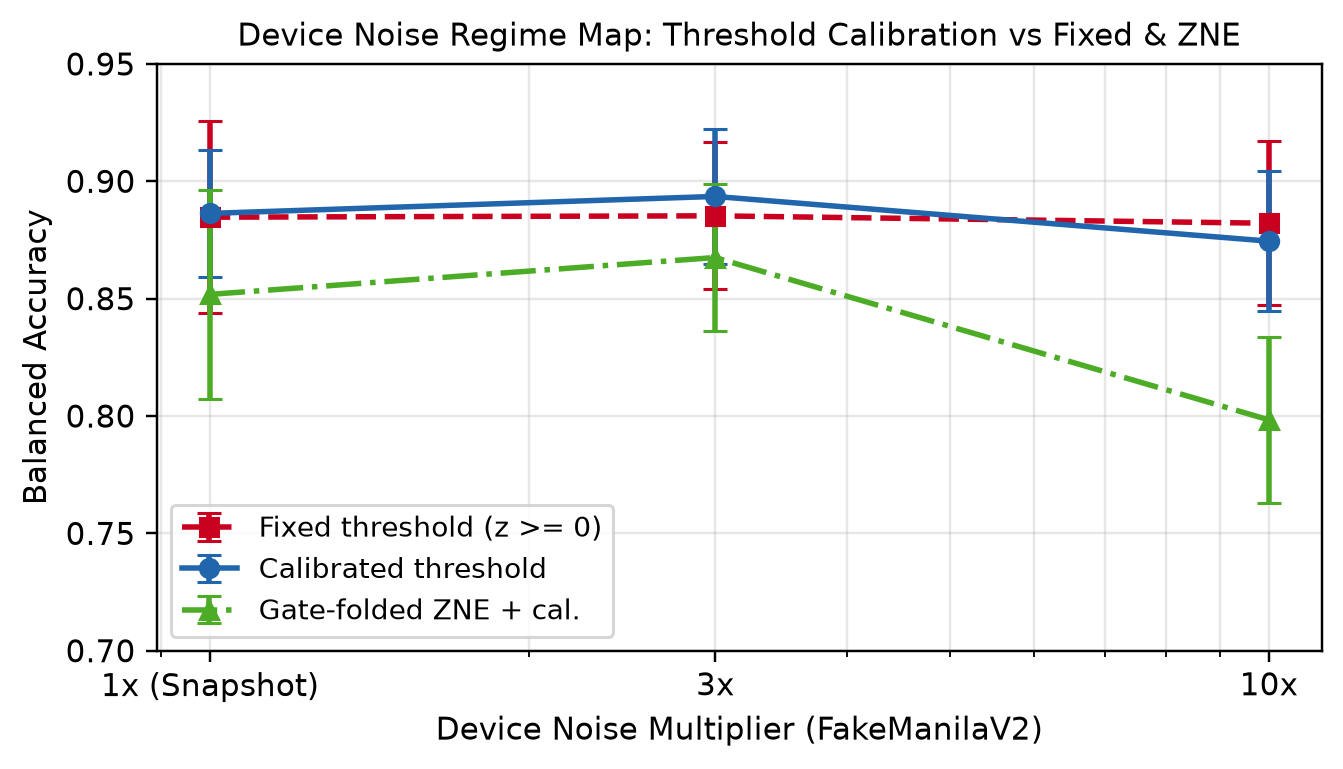
\includegraphics[width=0.98\columnwidth]{fake_manila_regime_map.png}
\caption{Exploratory noise-multiplier sweep using the saved IBM FakeManilaV2 snapshot noise model at multipliers $\times 1$, $\times 3$, and $\times 10$. This is a local simulation, not current device calibration or QPU data.}
\label{fig:regime-map}\end{figure}

\end{document}


